\documentclass[10pt,a4paper]{article}
\usepackage[margin=0.9in]{geometry}
\usepackage[T1]{fontenc}
\usepackage{lmodern}
\usepackage{microtype}
\usepackage{booktabs}
\usepackage{amsmath,amssymb}
\usepackage{algorithm}
\usepackage{algpseudocode}
\usepackage{caption}
\usepackage{xcolor}
\usepackage{tikz}
\usetikzlibrary{arrows.meta,positioning}
\usepackage{enumitem}
\usepackage{tabularx}
\usepackage[hidelinks]{hyperref}

\captionsetup{font=small,labelfont=bf,skip=4pt}
\setlist{itemsep=2pt,topsep=3pt}
\renewcommand{\arraystretch}{1.12}
\newcommand{\fmt}[1]{\texttt{#1}}
\algrenewcommand\algorithmiccomment[1]{\hfill{\small\color{black!60}$\triangleright$ #1}}

\title{\textbf{A Complete Single-Bit Flip Algorithm\\for Microscaling (MX) Tensors}}
\author{Peeyush Agarwal\\[2pt]
\small CS496 Undergraduate Project, Indian Institute of Technology Kanpur}
\date{26 October 2026}

\begin{document}
\maketitle

\begin{abstract}
\noindent This note gives the full algorithm for deciding what a single stored bit flip does to
an MX-quantised network, and explains every step. A flip turns into a wrong prediction only if
five things happen in a row: the bit really changes, the stored number changes, no check at
read time notices, the datapath carries the error forward, and the top-1 answer moves. The
algorithm follows that chain stage by stage. At the encoding stage it sorts every flip into
exactly one named case: eight for the shared scale (S0--S7) and fourteen for an element
(E0--E7 with sub-cases). The cases are checked in a fixed order, and an exhaustive test over
every code, every bit and every scale byte of all five element formats confirms that each flip
lands in exactly one case. Each stage is backed by the exhaustive ResNet8 weight campaigns
(483,904 faults in \fmt{e3m2}, 638,624 in \fmt{e4m3}), by re-injection under other datapaths,
and by exact counting on real activations.
\end{abstract}

\tableofcontents

%======================================================================
\section{Why an algorithm, and what ``every case'' means}

The first version of the case tree sorted a flip only by what it does to the stored number. That
explains the catastrophic faults well, but it says nothing about whether the flip could have
happened at all, whether a cheap check would catch it, or whether the hardware would pass it on.
The algorithm here adds those stages and keeps the case tree as stage~1.

``Every case is covered'' is meant in a strict sense:
\begin{enumerate}
  \item Every flip has exactly one case. The checks inside each stage run in a fixed order and
        the first that matches decides, so no flip has two cases and none has zero.
  \item This is checked by enumeration, not sampling. For each of the five element formats,
        every (code, bit) pair is classified: 2,048 pairs for the 8-bit formats, 384 for the 6-bit
        ones and 64 for \fmt{e2m1}. For the scale, all 256 bytes $\times$ 8 bits are classified,
        both for a zero block and for a non-zero one. The test
        \texttt{tests/test\_cases.py} asserts that each one maps to a single label through
        \texttt{mxfi.cases.label}.
  \item Cases that cannot happen in a clean tensor are still covered. A flip of a value that is
        already NaN (S7, E7) only happens after an earlier fault, but persistent weight faults do
        pile up between reloads, so the algorithm has to say what happens.
\end{enumerate}

%======================================================================
\section{Background: what is stored}

An MX tensor is cut into blocks of $K=32$ values. Each block stores one shared 8-bit scale byte
$X$ in E8M0 format and $K$ element codes in a small floating-point format. The value of element
$i$ is
\[
  x_i \;=\; 2^{X-127}\cdot v(c_i),
\]
where $v(c)$ is the value of element code $c$. E8M0 has no sign and no mantissa: bytes $0$--$254$
are the powers $2^{-127}$ to $2^{127}$, and byte $255$ is NaN. The OCP rule chooses
$X = \lfloor\log_2 \max_i|x_i|\rfloor - e_{\max} + 127$, so the largest element of every
non-zero block lands in the format's top binade. Table~\ref{tab:formats} lists the element
formats.

\begin{table}[h]
\centering
\caption{Element formats. ``Specials'' are codes that decode to NaN or $\pm$Inf.}
\label{tab:formats}
\begin{tabular}{lcccccl}
\toprule
format & bits & bias & $e_{\max}$ & largest value & smallest subnormal & special codes \\
\midrule
\fmt{e4m3} (FP8) & 8 & 7  & 8  & 448    & $2^{-9}$  & $\pm$NaN = S.1111.111 \\
\fmt{e5m2} (FP8) & 8 & 15 & 15 & 57,344 & $2^{-16}$ & $\pm$Inf, 6 NaNs (exponent 11111) \\
\fmt{e3m2} (FP6) & 6 & 3  & 4  & 28     & $2^{-4}$  & none \\
\fmt{e2m3} (FP6) & 6 & 1  & 2  & 7.5    & $2^{-3}$  & none \\
\fmt{e2m1} (FP4) & 4 & 1  & 2  & 6      & $2^{-1}$  & none \\
\bottomrule
\end{tabular}
\end{table}

Every element code belongs to one \emph{value class}: zero, subnormal (exponent field 0, mantissa
non-zero), normal, top binade (the largest finite exponent field), max (the largest finite
magnitude) or special. The class matters because the effect of a flip depends on where in the
range the value sits, not only on which bit flips.

%======================================================================
\section{The five-stage chain}

\begin{center}
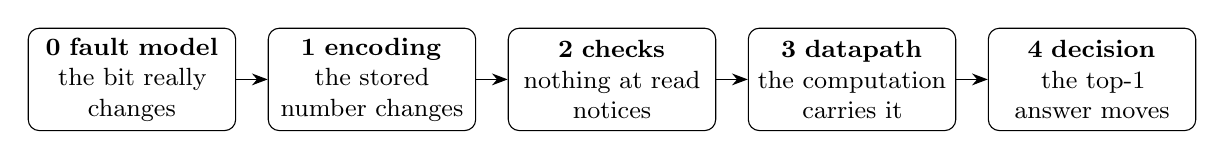
\begin{tikzpicture}[node distance=4mm,
  box/.style={draw,rounded corners,align=center,minimum height=13mm,text width=24mm,font=\small},
  arr/.style={-{Stealth[length=2mm]}}]
\node[box] (a) {\textbf{0 fault model}\\the bit really\\changes};
\node[box,right=of a] (b) {\textbf{1 encoding}\\the stored\\number changes};
\node[box,right=of b] (c) {\textbf{2 checks}\\nothing at read\\notices};
\node[box,right=of c] (d) {\textbf{3 datapath}\\the computation\\carries it};
\node[box,right=of d] (e) {\textbf{4 decision}\\the top-1\\answer moves};
\draw[arr] (a)--(b); \draw[arr] (b)--(c); \draw[arr] (c)--(d); \draw[arr] (d)--(e);
\end{tikzpicture}
\end{center}

A flip can stop at any stage. A stuck-at-1 fault on a bit that already holds 1 stops at stage~0;
a sign flip of $+0$ stops at stage~1; a NaN element code that a reader decodes as 0 stops at
stage~2; a NaN zeroed by a ReLU stops in stage~3 after erasing one channel; and a small finite
error usually stops at stage~4, because the prediction does not change. Stage~5 then adds up
the damage over all faults.

%======================================================================
\section{The algorithm}

Algorithm~\ref{alg:assess} is the whole procedure. Algorithms~\ref{alg:scale}
and~\ref{alg:element} are the two case trees of stage~1, written out in their checking order.

\begin{algorithm}[p]
\caption{\textsc{Assess}: what one fault does}
\label{alg:assess}
\small
\begin{algorithmic}[1]
\Require fault $f$ (site, bit or bit mask, kind), fault model $M$, datapath $P$
\Statex \textbf{Stage 0 --- does the bit actually change?}
\State $b \gets$ current value of the bit
\If{$f$ is stuck-at-$v$ \textbf{and} $b = v$} \Return F0 \textsc{masked} \EndIf
\If{$f$ hits a padding lane of the last block}
   \If{$P$ drops padding at decode} \Return F0 \textsc{masked}
   \Else\ continue; the lane meets a 0 input, so only a NaN/Inf code still matters
   \EndIf
\EndIf
\State $w(f) \gets \text{exposure}(f)\cdot p_M(b \to \lnot b)$
   \Comment{weights always resident; activations only while buffered}
\Statex \textbf{Stage 1 --- what does the stored number become?}
\If{$f$ is in a scale byte} \State $\text{case} \gets \textsc{ScaleCase}(f)$ \Comment{Alg.~\ref{alg:scale}}
\Else \State $\text{case} \gets \textsc{ElementCase}(f)$ \Comment{Alg.~\ref{alg:element}}
\EndIf
\State record context: $b$, $|\delta| = |v'-v|\cdot 2^{X-127}$, value class, one flip from NaN?,
       block maximum?, demotes the only top-binade element?, $X'$ in band?, zero-block scale
       (127 or 0), partial sum $P_B$, layer, input activity $a$
\Statex \textbf{Stage 2 --- does anything notice at read time?}
\If{element code is NaN/Inf} \Comment{D1}
   \If{guard G1 is on} decode it as 0 \Comment{E1 becomes ``one weight zeroed''}\EndIf
\EndIf
\If{$X'$ outside the tensor's clean band} \Comment{D2; D2a for weights: bit 7 set}
   \If{guard G2 is on \textbf{and} $X'$ above the band} treat the block as 0 \Comment{S1/S2/S3 $\to$ S6}\EndIf
\EndIf
\If{a non-zero block has no top-binade element} report; reload weights \Comment{D3}\EndIf
\Statex \textbf{Stage 3 --- what does the datapath do with it?}
\If{the value is NaN}
   \State zero inputs do not help: $\text{NaN}\cdot 0=\text{NaN}$
   \If{a NaN-zeroing ReLU follows} only that output channel is erased \Comment{P2}
   \Else\ NaN reaches the output \Comment{P1}
   \EndIf
\ElsIf{the value or the block's partial sum is $\pm$Inf}
   \State $+$Inf passes any ReLU; $-$Inf is zeroed by any ReLU \Comment{P3}
   \State $\text{Inf}\cdot 0 = \text{NaN}$; $(+\text{Inf}) + (-\text{Inf}) = \text{NaN}$
   \If{the accumulator saturates} the error stays finite and silent \Comment{P4}\EndIf
\Else
   \State output error $\approx \delta\cdot a$ (element) or $(2^{\Delta}-1)\cdot P_B$ (scale)
   \State zero inputs mask it fully (P5); ReLU masks part of a negative error (P6)
\EndIf
\If{activations are re-quantised} spread to block neighbours (P7); a NaN gives a NaN scale and 32 NaNs (P8)\EndIf
\Statex \textbf{Stage 4 --- does the answer change?}
\State outcome $\in$ \{O1 no change, O2 silent corruption, O3 non-finite output (caught by D4)\}
\State $\text{damage}(f) \gets$ share of images whose top-1 differs from the fault-free run
       (a non-finite logit row counts as a mismatch)
\Statex \textbf{Stage 5 --- aggregate and protect}
\State $\text{rate} = \sum_f w(f)\cdot\text{damage}(f)$;\quad silent rate = the part no check D1--D4 catches
\State protection order = bit positions sorted by damage per stored bit
\end{algorithmic}
\end{algorithm}

\begin{algorithm}[t]
\caption{\textsc{ScaleCase}: flip of scale byte $X$}
\label{alg:scale}
\small
\begin{algorithmic}[1]
\State $X' \gets X \oplus \text{mask}$;\quad $\Delta \gets X' - X$ \Comment{block multiplied by $2^{\Delta}$}
\If{$X' = 255$} \Return S1 \textsc{to NaN} \Comment{whole block NaN, zero blocks too}
\ElsIf{$X = 255$} \Return S7 \textsc{from NaN} \Comment{only after an earlier fault}
\ElsIf{every element is $\pm 0$} \Return S0 \textsc{zero block} \Comment{masked}
\ElsIf{$\max_i|v_i|\cdot 2^{X'-127} > \text{FP32}_{\max}$ \textbf{or} $\Delta = +128$} \Return S2 \textsc{overflow}
\ElsIf{$\Delta \ge 8$} \Return S3 \textsc{grow} $\times 256$ or more
\ElsIf{$\Delta > 0$} \Return S4 \textsc{grow} $\times 2$, $\times 4$, $\times 16$
\ElsIf{$\Delta \ge -2$} \Return S5 \textsc{shrink} $\div 2$, $\div 4$
\Else\ \Return S6 \textsc{erase} \Comment{$\div 16$ or more for one bit}
\EndIf
\end{algorithmic}
\end{algorithm}

\begin{algorithm}[t]
\caption{\textsc{ElementCase}: flip of element code $c$ with value $v$}
\label{alg:element}
\small
\begin{algorithmic}[1]
\State $c' \gets c \oplus \text{mask}$;\quad $v' \gets v(c')$
\If{$c$ is NaN/Inf} \Return E7 \textsc{from special}
\ElsIf{$c'$ is NaN/Inf} \Return E1 \textsc{to special} \Comment{always a $0\to1$ flip}
\ElsIf{sign bit} \Return E0 \textsc{masked} if $v=\pm 0$, else E2 \textsc{negate} \Comment{$|\delta| = 2|v|$}
\ElsIf{exponent bit $0\to 1$}
   \If{$v = 0$} \Return E3a \textsc{from zero}
   \ElsIf{$v$ subnormal} \Return E3b \textsc{subnormal}$\to$\textsc{normal}
   \Else\ \Return E3 \textsc{grow} $\times 2^{2^k}$
   \EndIf
\ElsIf{exponent bit $1\to 0$}
   \If{$v' = 0$} \Return E4a \textsc{to zero}
   \ElsIf{$v'$ subnormal} \Return E4b \textsc{normal}$\to$\textsc{subnormal}
   \Else\ \Return E4 \textsc{shrink} $\div 2^{2^k}$
   \EndIf
\ElsIf{mantissa bit $0\to 1$} \Return E5a \textsc{from zero} if $v = 0$, else E5 \textsc{grow}
\Else\ \Return E6a \textsc{to zero} if $v' = 0$, else E6 \textsc{shrink}
\EndIf
\end{algorithmic}
\end{algorithm}

%======================================================================
\section{Stage 0: the fault model}

\paragraph{Kinds of fault.} The algorithm covers a transient flip $0\to1$ (F1) or $1\to0$ (F2),
a stuck-at-1 (F3) or stuck-at-0 (F4) bit, and several bits of one word at once (F5). A stuck-at
fault on a bit that already holds the stuck value changes nothing (F0). So a stuck-at-1 fault
behaves exactly like the set of $0\to1$ flips, and a stuck-at-0 fault like the $1\to0$ flips.

\paragraph{Why direction matters.} Every catastrophic case needs a $0\to1$ flip. NaN codes, Inf
codes, scale byte 255 and the $+128$ scale jump are all runs of 1s, so a bit has to be \emph{set}
to reach them. In both exhaustive campaigns, all 2,468 (\fmt{e3m2}) and 10,321 (\fmt{e4m3})
catastrophic faults were $0\to1$.

\begin{table}[h]
\centering
\caption{Flip direction in the exhaustive ResNet8 weight campaigns (E27).}
\begin{tabular}{lcc}
\toprule
 & \fmt{e3m2} & \fmt{e4m3} \\
\midrule
stored bits that are 0 & 43\% & 40\% \\
share of damage from $0\to1$ flips (= stuck-at-1) & 87.5\% & 88.7\% \\
per-inference rate, $0\to1$ flips only & 0.00768 & 0.02089 \\
per-inference rate, $1\to0$ flips only & 0.00110 & 0.00267 \\
ratio & $7.0\times$ & $7.8\times$ \\
\bottomrule
\end{tabular}
\end{table}

So the failure rate is not a property of the format alone. A memory whose upsets are mostly
$1\to0$ would see about $8\times$ fewer failures than the symmetric model assumes. A stuck-at-0
bit is almost harmless; a stuck-at-1 bit is the dangerous kind.

\paragraph{Exposure.} Weights stay in memory for the whole deployment, so a weight fault is
persistent and hits every inference until the weights are reloaded. An activation is held only
while it sits in a buffer, so an activation fault is transient and hits one inference.

\paragraph{Padding lanes.} When a tensor's length is not a multiple of 32, the last block is
padded. A flip in a padding lane is masked if decode drops the padding, which is what
\texttt{mxfi} does. Hardware that multiplies the whole block instead pairs the lane with a 0
input. A finite error is still masked, but a NaN or Inf code is not, since $\text{NaN}\cdot 0$ and
$\text{Inf}\cdot 0$ are both NaN.

\paragraph{Several bits of one word.} With $\Delta = X'-X$, the scale tree holds as written: a
mask that gives $\Delta=-3$ is S6 ($\div 8$). For an element, the first two checks (from or to a
special code) still hold. When the flipped bits span fields or flip in both directions,
``field'' and ``direction'' no longer mean anything, so the case is described by the value-class
change and $|\delta|$ instead. Flips within one word were measured earlier to be sub-additive (E21).

%======================================================================
\section{Stage 1: the scale case tree}

\paragraph{The key fact.} Flipping bit $j$ of the scale byte changes $X$ by exactly $+2^j$ if the
bit was 0 and $-2^j$ if it was 1. So the block is multiplied by $2^{\pm 2^j}$, and how far it
moves is fixed by the bit position alone. The value of $X$ only decides the direction and whether
a boundary (255, or the FP32 range) is crossed. For a typical weight scale $X=117$
(\texttt{01110101}):

\begin{center}
\begin{tabular}{lcccccccc}
\toprule
bit $j$ & 0 & 1 & 2 & 3 & 4 & 5 & 6 & 7 \\
\midrule
$\Delta$ & $-1$ & $+2$ & $-4$ & $+8$ & $-16$ & $-32$ & $-64$ & $+128$ \\
case & S5 & S4 & S6 & S3 & S6 & S6 & S6 & S2 \\
\bottomrule
\end{tabular}
\end{center}

\paragraph{The cases, in checking order.}
\begin{description}[leftmargin=1.2em,style=nextline]
  \item[S1 to NaN ($X'=255$).] Only bytes with seven 1s can reach 255. The whole block decodes to
        NaN, zeros included, since $0\cdot\text{NaN}=\text{NaN}$. That is why this check comes
        before the zero-block check. In the weight campaigns no clean scale had seven 1s, so S1
        never occurred there; it appears in activations, whose scales sit near 127 (0.2--1.0\% of
        activation scale flips in FP6/FP4).
  \item[S7 from NaN ($X=255$).] The block was already NaN after an earlier fault; any flip
        makes it finite again. This is a repair, not a shrink, so it is its own case.
  \item[S0 zero block.] Every element is $\pm 0$, so any finite scale gives 0. Masked.
  \item[S2 overflow.] The block leaves the FP32 range, either at decode or (for $\Delta=+128$) in
        the accumulation that reads it. Whether it really becomes Inf is a stage-3 question; see
        Section~\ref{sec:datapath}.
  \item[S3 grow $\times256$ or more ($\Delta\ge 8$).] Finite but huge: mean damage 0.74--0.76.
  \item[S4 grow ($0<\Delta<8$).] $\times2$, $\times4$ or $\times16$. Wide spread: the median
        damage is 0.04--0.06, but the 90th percentile is 0.33--0.43, depending on the block's
        partial sum $P_B$.
  \item[S5 shrink ($-2\le\Delta<0$).] $\div2$ or $\div4$. Mild.
  \item[S6 erase ($\Delta\le -3$).] The block shrinks $16\times$ or more and is effectively deleted.
\end{description}

%======================================================================
\section{Stage 1: the element case tree}

The case of an element flip is the field of the bit, the direction of the flip and the
value-class transition it causes. Worked examples in \fmt{e4m3} (bias 7):

\begin{center}
\begin{tabular}{lllll}
\toprule
case & before & bit flipped & after & effect \\
\midrule
E3 grow & $1.0$ = 0.0111.000 & exponent bit 3, $0\to1$ & 0.1111.000 = 256 & $\times 2^{8}$ \\
E4 shrink & $1.0$ = 0.0111.000 & exponent bit 2, $1\to0$ & 0.0011.000 = $1/16$ & $\div 2^{4}$ \\
E4b normal$\to$sub & $1.5\cdot2^{-6}$ = 0.0001.100 & exponent bit 0 & 0.0000.100 = $2^{-7}$ & $\div 3$ \\
E1 to NaN & 448 = 0.1111.110 & mantissa bit 0 & 0.1111.111 = NaN & non-finite \\
E2 negate & $v$ & sign & $-v$ & $|\delta| = 2|v|$ \\
E0 masked & $+0$ & sign & $-0$ & none \\
\bottomrule
\end{tabular}
\end{center}

\begin{description}[leftmargin=1.2em,style=nextline]
  \item[E7 from special.] The code was already NaN/Inf. In a clean tensor this never occurs; in
        \fmt{e5m2} a mantissa flip of an Inf code gives NaN.
  \item[E1 to special.] The new code is NaN or Inf. Every such flip is $0\to1$. In \fmt{e4m3}
        only the seven magnitudes 1.875, 30, 120, 240, 352, 416 and 448 are one flip from NaN, and
        both exponent and mantissa bits can do it. In \fmt{e5m2} only exponent bits can, and they can
        reach $\pm$Inf (E1i) as well as NaN (E1n). \fmt{e3m2}, \fmt{e2m3} and \fmt{e2m1} have no
        special codes, so E1 and E7 never occur in them. Mean damage of E1 in the weight campaign:
        1.0 for every single fault.
  \item[E0 / E2 sign.] A sign flip of zero is masked; of anything else it negates the value.
        Where a format puts its special codes is a parameter: in an FNUZ format the $-0$ pattern
        1.0000.000 is NaN, so the sign flip of $+0$ becomes E1.
  \item[E3 / E4 exponent.] Flipping exponent bit $k$ between two normal values multiplies or
        divides by exactly $2^{2^k}$. The sub-cases are the boundary crossings: from zero (E3a),
        subnormal to normal (E3b), to zero (E4a), normal to subnormal (E4b).
  \item[E5 / E6 mantissa.] Smaller changes inside one binade, with the zero crossings E5a and E6a.
\end{description}

\paragraph{The case is not enough for finite flips.} Table~\ref{tab:r2} shows how much of the
measured damage each description explains (held-out $R^2$, two-fold). The case decides the
catastrophic part almost completely, but within ordinary finite element flips it explains only
2--5\%. What matters there is the size of the error reaching the next layer:
$|v'-v|\cdot 2^{X-127}$ times the activity of the input the weight multiplies. The block's
scale $X$ is a factor the first version ignored.

\begin{table}[h]
\centering
\caption{Variance of damage explained (E27).}
\label{tab:r2}
\begin{tabular}{lcc}
\toprule
model & all faults (\fmt{e3m2} / \fmt{e4m3}) & finite element flips (\fmt{e3m2} / \fmt{e4m3}) \\
\midrule
site only & 0.22 / 0.09 & 0 / -- \\
+ case & 0.91 / 0.97 & 0.02 / 0.05 \\
+ bit position & 0.92 / 0.98 & 0.02 / 0.06 \\
+ layer & 0.94 / 0.98 & 0.19 / 0.21 \\
+ size of the weight error & 0.94 / 0.98 & 0.54 / 0.54 \\
size $\times$ input activity instead & 0.94 / 0.98 & 0.67 / 0.64 \\
+ sign of the error & 0.94 / 0.98 & 0.70 / 0.66 \\
\bottomrule
\end{tabular}
\end{table}

\paragraph{Context recorded with each case.} Flip direction; value class; one flip from NaN;
whether the element is its block's maximum (5\% of \fmt{e3m2} element faults, 21\% of their
damage); whether it demotes the block's only top-binade element; whether $X'$ is in the clean
band; the zero-block scale encoding (a from-zero flip in a block with $X=127$ gives a value up to
$\pm2$, but with $X=0$ it gives about $2^{-126}$); the special-code placement; layer; error size;
input activity.

\paragraph{Measured damage by case.} Table~\ref{tab:cases} gives the exhaustive weight results.

\begin{table}[h]
\centering
\caption{Mean damage per case, exhaustive ResNet8 weight campaigns (E25). Damage share is the
part of the total per-inference rate the case causes.}
\label{tab:cases}
\begin{tabular}{llrrrr}
\toprule
 & & \multicolumn{2}{c}{\fmt{e3m2}} & \multicolumn{2}{c}{\fmt{e4m3}} \\
\cmidrule(lr){3-4}\cmidrule(lr){5-6}
label & case & mean damage & damage share & mean damage & damage share \\
\midrule
S2 & scale overflow     & 0.974 & 56.5\% & 0.978 & 16.0\% \\
S3 & scale grow large   & 0.742 & 10.4\% & 0.756 & 12.4\% \\
S4 & scale grow small   & 0.146 & 14.6\% & 0.111 & 2.2\% \\
S5 & scale shrink       & 0.011 & 0.7\%  & 0.017 & 0.3\% \\
S6 & scale erase        & 0.024 & 5.5\%  & 0.029 & 1.8\% \\
E1 & element to NaN     & --    & --     & 1.000 & 52.2\% \\
E2 & negate             & 0.0030 & 5.5\% & 0.0073 & 3.8\% \\
E3 & exponent grow      & 0.0017 & 3.1\% & 0.0055 & 2.9\% \\
E4 & exponent shrink    & 0.0010 & 3.2\% & 0.0043 & 6.3\% \\
E5 & mantissa grow      & 0.0002 & 0.3\% & 0.0015 & 1.2\% \\
E6 & mantissa shrink    & 0.0001 & 0.2\% & 0.0012 & 0.9\% \\
E0, E3--6a/b & boundary cases & $\le$0.00013 & $<$0.1\% & $\le$0.00013 & $<$0.1\% \\
\bottomrule
\end{tabular}
\end{table}

\paragraph{Activations behave differently.} Counting over real inputs of ResNet8 and RepVGG-A0:
40--55\% of activation values are exactly 0, so 5--15\% of element flips are masked sign flips
and 33--48\% are flips from zero to a tiny value. In OCP \fmt{e4m3} 0.7--1.2\% of activation
element flips reach NaN (3.5--5.2\% in \fmt{e5m2}). With FNUZ-style placement it would be
5.0--6.8\%, because zero is the most common value and its sign flip would be NaN.

%======================================================================
\section{Stage 2: free checks and guards}

A clean OCP MX tensor obeys three invariants, and checking them needs no extra memory:
\begin{description}[leftmargin=1.2em]
  \item[D1] No element code is NaN/Inf. Guard \textbf{G1}: decode such a code as 0.
  \item[D2] Every scale lies in the tensor's clean band (known offline for weights, calibrated on
        a few inputs for activations). For weights, D2a is simpler: no clean weight scale has
        bit~7 set. Guard \textbf{G2}: a block whose scale is above the band is treated as 0.
  \item[D3] Every non-zero block has an element in the top binade.
\end{description}
D4, a check that the logits are finite, sits at the output and catches what reaches it as NaN/Inf.

\begin{table}[h]
\centering
\caption{Share of damage each check flags, and the effect of the guards (E27).}
\begin{tabular}{lcc}
\toprule
 & \fmt{e3m2} & \fmt{e4m3} \\
\midrule
D1 element code is NaN/Inf & -- & 52.2\% \\
D2a scale bit 7 set & 56.5\% & 16.0\% \\
D2b scale outside the clean band & 85.7\% & 32.1\% \\
D3 lost top-binade element & 0.1\% & 0.2\% \\
D1 + D2b + D3 at read (3.5\% / 4.1\% of faults) & 85.8\% & 84.5\% \\
D4 non-finite output & 56.2\% & 68.1\% \\
\midrule
rate, no guard & 0.00878 & 0.0236 \\
rate, G2 only & 0.00206 ($4.3\times$) & 0.0168 ($1.4\times$) \\
rate, G1 only & -- & 0.0113 ($2.1\times$) \\
rate, G1 + G2 & 0.00206 ($4.3\times$) & 0.00454 ($5.2\times$) \\
silent rate left after all checks & 0.00124 & 0.00364 \\
\bottomrule
\end{tabular}
\end{table}

G2's effect is exact: a block treated as 0 has the measured damage of the same block's
$\div2^{64}$ flip. G1 was measured by injecting 2,000 E1 faults with the code decoded as 0; mean
damage fell from 1.0 to 0.0064. For activations, a band calibrated on 10 images had 0.01\% false
alarms on 10 others and caught every flip of scale bits 3--7.

%======================================================================
\section{Stage 3: the datapath}
\label{sec:datapath}

The same flip can be catastrophic or mild depending on the hardware. The rules:

\begin{description}[leftmargin=1.2em,style=nextline]
  \item[P1 / P2 NaN.] $\text{NaN}\cdot0=\text{NaN}$, so zero inputs do not mask a NaN weight. The
        PyTorch ReLU passes NaN on (P1). A NaN-zeroing ReLU ($x>0\;?\;x:0$, IEEE maxNum) turns it
        into ``this output channel is erased'' (P2), except in the last layer, where no ReLU
        follows. Re-injected: E1 mean damage 1.00 with a NaN-passing ReLU, 0.085 with a
        NaN-zeroing one, 0.0064 with the read guard G1.
  \item[P3 overflow.] $+$Inf passes any ReLU; $-$Inf is zeroed by any ReLU (a batch norm with
        negative $\gamma$ can flip the sign first). $\text{Inf}\cdot0=\text{NaN}$, and $+$Inf and
        $-$Inf meeting in a later sum give NaN.
  \item[S2 in detail.] $\Delta=+128$ multiplies the block's partial sum by $2^{128}$, which
        overflows FP32 only when $|P_B|>1$. In both campaigns 98.7\% of these flips gave
        non-finite outputs, not 100\%. A negative partial sum ($-$Inf, zeroed by ReLU) and a
        partial sum below 1 can both leave the output finite; the two were not separated.
        Under a NaN-zeroing ReLU S2's damage stays at 0.97, because $+$Inf is not NaN, so only a
        scale check (D2/G2) helps.
  \item[P4 saturation.] A saturating accumulator turns overflow into a silent finite error.
  \item[P5 zero inputs.] A finite weight error that only multiplies zeros changes nothing.
        (ResNet8 had no input channel that was zero on all 200 images, so this was not observed.)
  \item[P6 ReLU asymmetry.] In hidden layers, an error that raises the pre-activation is
        1.07--1.12$\times$ worse than one that lowers it, up to 1.2--1.4$\times$ at the largest
        errors, because a positive error can switch a unit on.
  \item[P7 re-quantisation.] In an all-MX pipeline every layer's input is re-encoded. An error
        that makes a value $r\times$ its block maximum raises the block's scale, and neighbours far
        below the new maximum are flushed to 0. Share of non-zero neighbours flushed:
\end{description}

\begin{center}
\begin{tabular}{lccccc}
\toprule
format & $r=2$ & $r=4$ & $r=16$ & $r=256$ & $r=65536$ \\
\midrule
\fmt{e5m2} & 0 & 0 & 0 & 0 & 0 \\
\fmt{e4m3} & 0 & 0 & 0.01\% & 0.1\% & 29\% \\
\fmt{e3m2} & 0.5\% & 0.9\% & 3.9\% & 55\% & 100\% \\
\fmt{e2m3} & 3.7\% & 7.4\% & 28\% & 100\% & 100\% \\
\fmt{e2m1} & 15\% & 29\% & 91\% & 100\% & 100\% \\
\bottomrule
\end{tabular}
\end{center}

\begin{description}[leftmargin=1.2em,style=nextline]
  \item[P8 NaN at re-quantisation.] A NaN reaching re-quantisation becomes a NaN scale and so 32
        NaNs. What an Inf does there depends on the implementation (a NaN scale, or saturation to
        the largest code).
\end{description}

%======================================================================
\section{Stage 4: the decision}

Damage is the share of test images whose top-1 prediction differs from the fault-free run. An
image whose logit row is not finite is counted as class $-1$, a mismatch, so a NaN that reaches
every image gives damage exactly 1. Each fault ends in one of three outcomes:

\begin{center}
\begin{tabular}{lcc}
\toprule
outcome & \fmt{e3m2} rate (share) & \fmt{e4m3} rate (share) \\
\midrule
O1 no change & 0 & 0 \\
O2 silent corruption & 0.00384 (44\%) & 0.00750 (32\%) \\
O3 non-finite output, caught by D4 & 0.00494 (56\%) & 0.01606 (68\%) \\
\bottomrule
\end{tabular}
\end{center}

For a weight fault one caught NaN output is enough: the fault is persistent, so the system can
reload the weights, and the fault becomes a detected error instead of a silent one. Most of
\fmt{e4m3}'s extra damage over \fmt{e3m2} is this detectable kind.

%======================================================================
\section{Stage 5: aggregate and protect}

The per-inference rate is $\sum_f w(f)\cdot\text{damage}(f)$, and its silent part is what no
check D1--D4 catches. Sorting bit positions by damage per stored bit gives the protection order:
\begin{itemize}
  \item \fmt{e3m2}: scale bit 7 is 0.5\% of storage and 57\% of damage. Scale bits 7, 3, 2 and 1
        are 2\% of storage and 83\% of damage, so protecting by bit position works well.
  \item \fmt{e4m3}: 27\% of storage is needed for half the damage, because NaN damage is spread
        over every element bit. Protecting by bit position works badly; G1 plus G2 do far better
        at no storage cost.
\end{itemize}

%======================================================================
\section{Proof of coverage}

Table~\ref{tab:coverage} counts how many (code, bit) pairs of each format fall in each element
case. Every row sums to the full code space ($2^{\text{width}}\times\text{width}$). For the scale,
the 4,096 (byte, bit, zero block or not) combinations split into S0 2,032, S1 16, S2 127, S3 508,
S4 381, S5 254, S6 762 and S7 16. All eight scale cases and all fourteen element labels occur,
and none is left over.

\begin{table}[h]
\centering
\caption{Exhaustive enumeration of element flips by case.}
\label{tab:coverage}
\small\setlength{\tabcolsep}{2.6pt}
\begin{tabular}{lrrrrrrrrrrrrrrr}
\toprule
format & E0 & E1 & E2 & E3 & E3a & E3b & E4 & E4a & E4b & E5 & E5a & E6 & E6a & E7 & total \\
\midrule
\fmt{e4m3} & 2 & 14 & 252 & 440 & 8 & 56 & 440 & 8 & 56 & 372 & 6 & 372 & 6 & 16 & 2048 \\
\fmt{e5m2} & 2 & 40 & 246 & 560 & 10 & 30 & 560 & 10 & 30 & 244 & 4 & 244 & 4 & 64 & 2048 \\
\fmt{e3m2} & 2 & 0 & 62 & 72 & 6 & 18 & 72 & 6 & 18 & 60 & 4 & 60 & 4 & 0 & 384 \\
\fmt{e2m3} & 2 & 0 & 62 & 32 & 4 & 28 & 32 & 4 & 28 & 90 & 6 & 90 & 6 & 0 & 384 \\
\fmt{e2m1} & 2 & 0 & 14 & 8 & 4 & 4 & 8 & 4 & 4 & 6 & 2 & 6 & 2 & 0 & 64 \\
\bottomrule
\end{tabular}
\end{table}

\begin{table}[h]
\centering
\caption{All cases, by stage.}
\begin{tabularx}{\linewidth}{lX}
\toprule
stage & cases \\
\midrule
0 fault model & F0 masked (stuck value already stored, or padding dropped) $\cdot$ F1 transient $0\to1$
  $\cdot$ F2 transient $1\to0$ $\cdot$ F3 stuck-at-1 $\cdot$ F4 stuck-at-0 $\cdot$ F5 several bits of one word \\
1 scale & S0 zero block $\cdot$ S1 to NaN $\cdot$ S2 overflow $\cdot$ S3 grow $\ge\times256$ $\cdot$
  S4 grow $\times2/\times4/\times16$ $\cdot$ S5 shrink $\div2/\div4$ $\cdot$ S6 erase $\cdot$ S7 from NaN \\
1 element & E0 masked $\cdot$ E1 to NaN/Inf $\cdot$ E2 negate $\cdot$ E3 exponent grow (E3a, E3b) $\cdot$
  E4 exponent shrink (E4a, E4b) $\cdot$ E5 mantissa grow (E5a) $\cdot$ E6 mantissa shrink (E6a) $\cdot$ E7 from NaN/Inf \\
2 checks & D1 special code $\to$ G1 $\cdot$ D2 scale out of band (D2a bit 7) $\to$ G2 $\cdot$ D3 lost block maximum $\cdot$ D4 output check \\
3 datapath & P1 NaN propagates $\cdot$ P2 NaN zeroed by ReLU $\cdot$ P3 overflow to $\pm$Inf $\cdot$
  P4 saturation $\cdot$ P5 zero inputs mask finite errors $\cdot$ P6 ReLU asymmetry $\cdot$
  P7 re-quantisation spreads errors $\cdot$ P8 NaN block $\to$ 32 NaNs \\
4 decision & O1 no change $\cdot$ O2 silent corruption $\cdot$ O3 non-finite output \\
\bottomrule
\end{tabularx}
\end{table}

%======================================================================
\section{What the algorithm does not cover}

\begin{itemize}
  \item Faults outside stored MX values: accumulators, partial sums, biases, normalisation
        parameters, control logic and addressing (a block paired with the wrong scale). The
        element tree is format-generic, so FP32/BF16 values could use it with their own special
        codes, but this was not measured.
  \item Faults piling up across words in weight memory between reloads (S7 and E7 say what one
        more flip does, but the build-up itself was not measured).
  \item Damage under a saturating accumulator, an FP16 accumulator, or a full MX activation
        pipeline end to end. P3, P4, P7 and P8 are rules from the arithmetic here, not injected
        measurements, and the same holds for the $\pm$Inf and padding-lane rules.
  \item One network measured exhaustively (ResNet8, width 16). Activation results cover ResNet8
        and RepVGG-A0.
\end{itemize}

\paragraph{Reproducing.} Code is in \texttt{mxfi/cases.py}; experiments in
\texttt{experiments/e25}--\texttt{e28}; raw output in \texttt{results/}.
\begin{verbatim}
python -m pytest tests/test_cases.py -q     # the coverage test
python -m experiments.e25_flip_cases
python -m experiments.e26_datapath          # about 20 min on CPU
python -m experiments.e27_fault_model       # after e25 and e26
python -m experiments.e28_activation_cases
\end{verbatim}

\end{document}
